\documentclass[a4paper,12pt]{article}

\usepackage[T1]{fontenc}
\usepackage[utf8]{inputenc}
%\usepackage{mathtools}
\usepackage{graphicx}
\usepackage[margin=1in]{geometry}
\usepackage[spanish,es-noquoting]{babel}
\usepackage{hyperref}
\usepackage{fancyhdr}
\usepackage{incgraph,tikz}
\usepackage{caption}
\usepackage{subcaption}
\usepackage{amsfonts}
\usepackage{babel}
\usepackage{color}
\usepackage{listings}
\usepackage{float}
\usepackage{tikz}
\usepackage{adjustbox}
\usepackage{natbib}
\usepackage{subcaption}
\usepackage{cleveref}
\usepackage{color}
\usepackage{ulem}
\usepackage{listings}
\usepackage{minted}
\usepackage{url}
\lstset{ %
basicstyle=\footnotesize,       % the size of the fonts that are used for the code
numbers=none,                   % where to put the line-numbers
numberstyle=\footnotesize,      % the size of the fonts that are used for the line-numbers
stepnumber=1,                   % the step between two line-numbers. If it is 1 each line will be numbered
numbersep=10pt,                  % how far the line-numbers are from the code
backgroundcolor=\color{white},  % choose the background color. You must add \usepackage{color}
showspaces=false,               % show spaces adding particular underscores
showstringspaces=false,         % underline spaces within strings
showtabs=false,                 % show tabs within strings adding particular underscores
frame=single,           % adds a frame around the code
tabsize=4,          % sets default tabsize to 2 spaces
captionpos=b,           % sets the caption-position to bottom
breaklines=true,        % sets automatic line breaking
breakatwhitespace=false,    % sets if automatic breaks should only happen at whitespace
escapeinside={\%*}{*)}          % if you want to add a comment within your code
}
\usepackage{titling}
\newcommand{\subtitle}[1]{%
	\posttitle{%
		\par\end{center}
	\begin{center}\large#1\end{center}
	\vskip0.5em}%
}

\usetikzlibrary{arrows}

\captionsetup[subfigure]{subrefformat=simple,labelformat=simple}

\renewcommand{\lstlistingname}{Salida}
\renewcommand\spanishtablename{Tabla}
\renewcommand{\figurename}{Gráfico}
\renewcommand\thesubfigure{(\alph{subfigure})}
\renewcommand{\baselinestretch}{1.2} 

\makeatletter
\def\verbatim{\small\@verbatim \frenchspacing\@vobeyspaces \@xverbatim}
\makeatother

\pagestyle{fancy}

\restylefloat{table}

\title{Burger Bot}
\subtitle{Final Programación Funcional}
\author{Fermin Gomez}
\lhead{Final Programación Funcional}
\rhead{ITBA}

\begin{document}

\maketitle

\begin{figure}[H]
	\centering
	
\includegraphics[width=0.7\linewidth]{itba}
\end{figure}

\pagebreak

\tableofcontents

\pagebreak

\section{Introducción}

El contexto actual de pandemia genera una necesidad en la sociedad de reinventarse. En el caso particular de la hamburguesería Arredondo para disminuir la circulación y contacto entre personas en la sucursal se optó por tomar los pedidos de los clientes vía WhatsApp. 
\\
La solución adoptada necesita de la adquisición de por lo menos un número telefónico y un smartphone, el cual sería utilizado por por un empleado para tomar los pedidos y hacer entrega de la comanda a la cocina. La disponibilidad del mismo es esencial para brindar un buen servicio. 
\\
El enfoque tomado consiste en tomar la propuesta de Arredondo y convertirla en una de mayor eficiencia en términos de costo, recursos, tiempo, empleados y que maximice las ventas.  

\section{Descripción de la Solución}

Mi propuesta comienza con la automatización de la toma de pedidos mediante la implementación de un chatbot. Se busca mantener una alta disponibilidad para tomar pedidos y evitar la necesidad de emplear a una o más personas para realizar el trabajo.
El chatbot permitirá al usuario cliente armar las hamburguesas según sus preferencias, permitiéndoles elegir el tamaño, ingredientes adicionales y salsas. Una vez creada la hamburguesa se la agregaría a la orden del cliente. En cualquier momento se podrá visualizar las hamburguesas de la orden junto con sus respectivos precios,  quitar una hamburguesa de la orden, como también enviar el pedido al restaurante. 
\\
Para mantener registro de los pedidos enviados por los clientes se implementará una aplicación web. Esta permitirá a los empleados visualizar los pedidos en curso y marcarlos como completados, cómo también realizar búsquedas aplicando filtros. 
\\
Como requerimiento mínimo se necesitaría de una computadora sobre la cual correría el bot y además debería estar a disposición del personal para acceder a la aplicación web.

\pagebreak

\subsection{Chatbot}
Es importante que tanto los clientes jóvenes como los adultos que atienden la hamburguesería puedan realizar un pedido, no queremos que se pierda un sector de la clientela regular. Por ello el proceso para realizar el pedido debe mantenerse sencillo e intuitivo.

\begin{figure}[H]
	\centering
	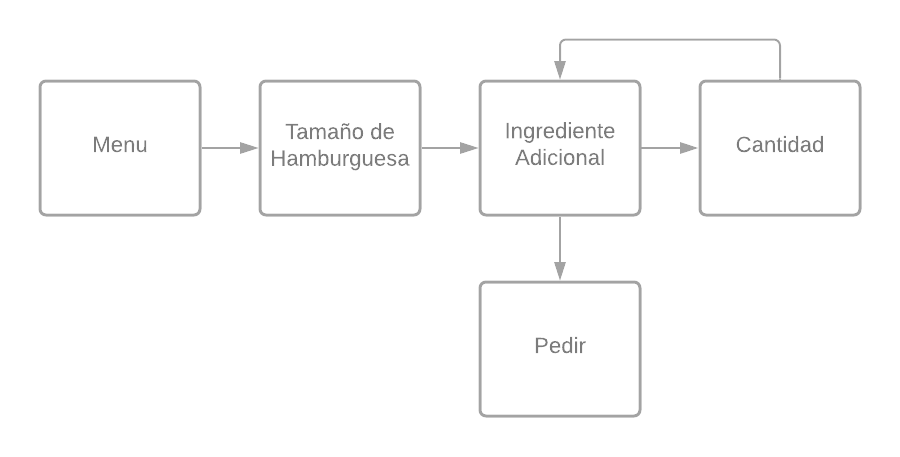
\includegraphics[width=1.0\linewidth]{diagrama-flujo.png}
\end{figure}

Al iniciar una conversación con el chatbot podemos comenzar agregando hamburguesas a la orden ejecutando el comando
\color{blue}\uline{\textbackslash menu}\color{black}. 
\\
A continuación detallaremos las fases del proceso de armado de la hamburguesa.

\begin{itemize}
	
	\item \textbf{Fase 1}: El primer paso consiste en seleccionar el tamaño deseado para nuestra hamburguesa, puede ser simple, doble o triple.
	
	\item \textbf{Fase 2}: Una vez seleccionado el tamaño de la hamburguesa procedemos a elegir los ingredientes adicionales, entre ellos: queso, pepinos, tomate, lechuga, salsa, etc. 
	
	\item \textbf{Fase 3}: Una vez seleccionado el ingrediente deseado procedemos a elegir la cantidad deseada del mismo. Una vez seleccionada la cantidad volveremos a la Fase 2, lo cual nos permite seguir agregando otros ingredientes.
	
	\item \textbf{Fase 4}: Una vez creada la hamburguesa deseada, es decir no se necesita agregar más ingredientes la agregamos a nuestra orden.	
	
\end{itemize}

Otro de los comandos disponibles es \color{blue}\uline{\textbackslash show}\color{black}
que nos permite visualizar las hamburguesas en la orden. En el caso de que se desee quitar un producto se encuentra el comando
\color{blue}\uline{\textbackslash remove <id>}\color{black}
, que recibe como parámetro el identificador de la hamburguesa que se desea quitar de la orden. Una vez agregadas todas las hamburguesas a nuestro pedido ejecutando el comando 
\color{blue}\uline{\textbackslash confirm}\color{black} 
enviamos la orden al restaurante.
\\
El proceso se ideó con el objetivo de agilizar la manera de pedir comida y guiar al usuario por las distintas fases. En todo momento se puede ejecutar el comando 
\color{blue}\uline{\textbackslash help}\color{black}
el cual aporta ayuda sobre los distintos comandos y cómo comenzar un pedido.

\subsection{Aplicación Web}

El personal del restaurante podrá visualizar y mantener registro de los pedidos de los clientes accediendo a la aplicación web disponible en la red local ingresando a 
\color{blue}\uline{http://localhost:3000}\color{black}.
\\
Bajo la sección “Pending Orders” se podrá realizar un seguimiento de las órdenes enviadas por los clientes que aún no fueron completadas. Las mismas se encuentran ordenadas desde la más antigua a la más reciente, dándole prioridad a aquellos que realizaron antes su pedido.

\begin{figure}[H]
	\centering
	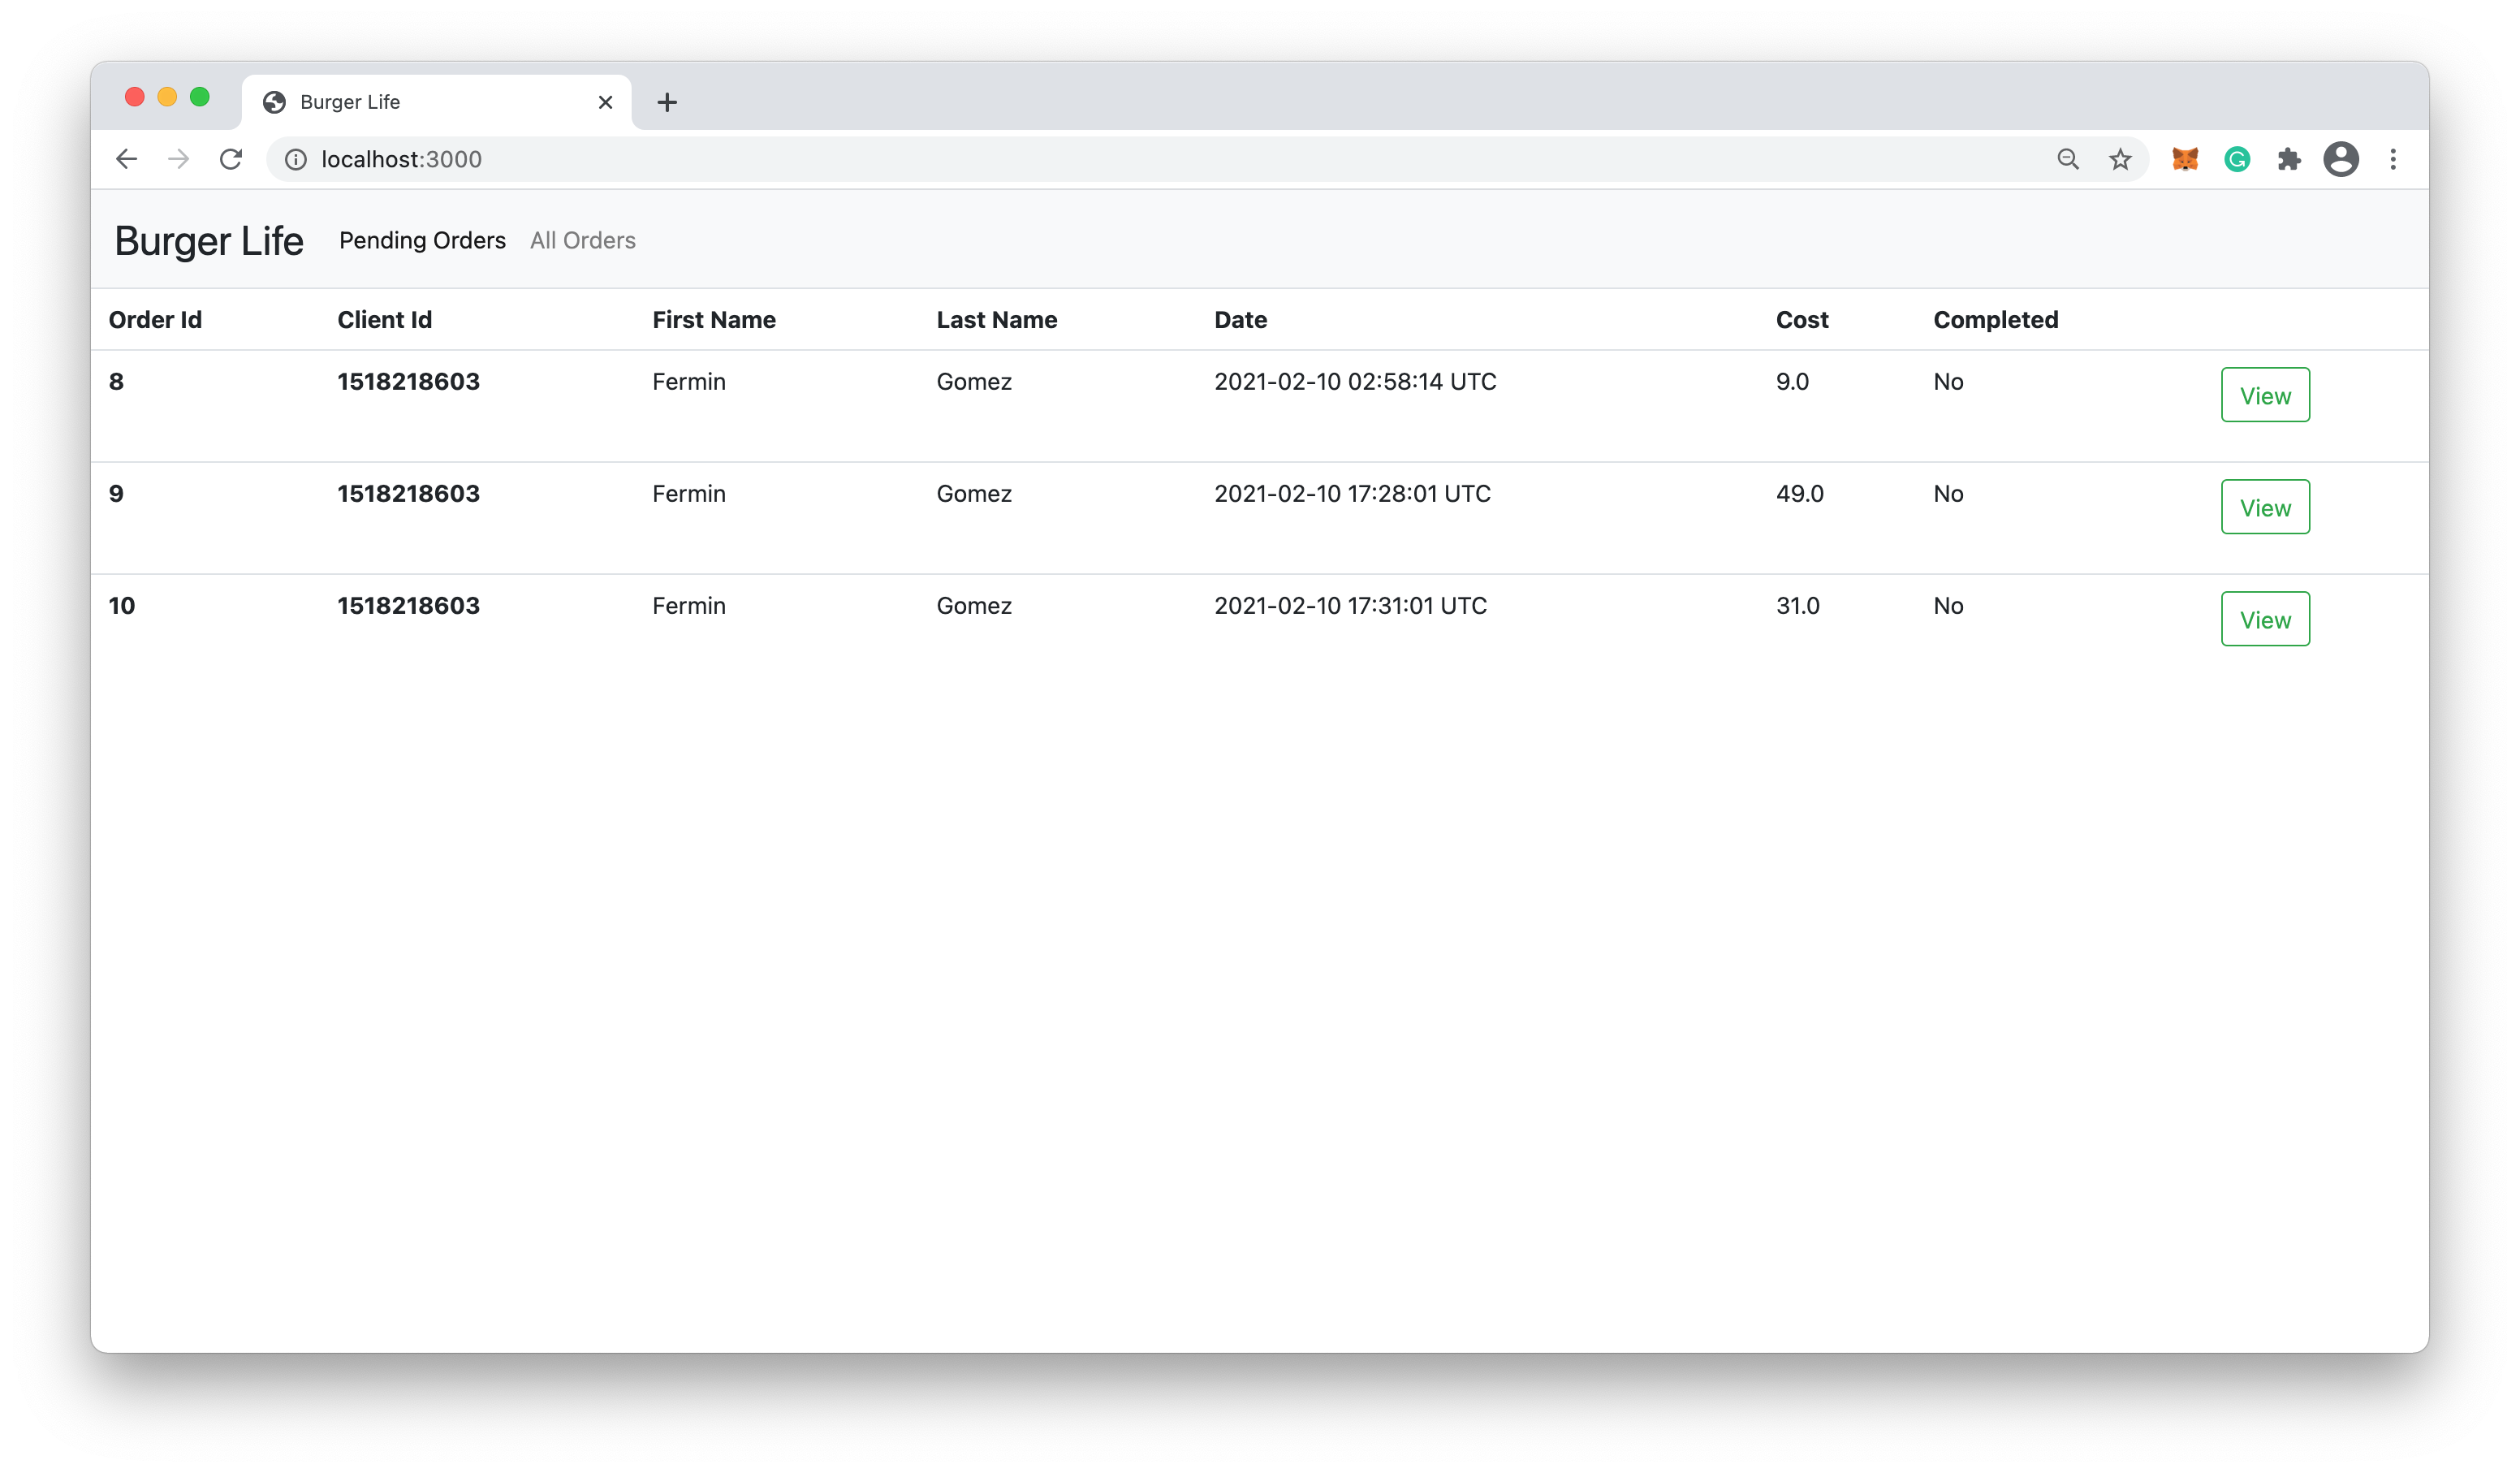
\includegraphics[width=1.0\linewidth]{webapp-pending-orders}
\end{figure}

Clickeando en el botón “View” de una orden podremos ver las hamburguesas encargadas por el cliente. Una vez enviada la comanda hacia la cocina y finalizada la orden el empleado a cargo deberá marcarla como completada clickeando en el botón “Mark as Completed”.

\begin{figure}[H]
	\centering
	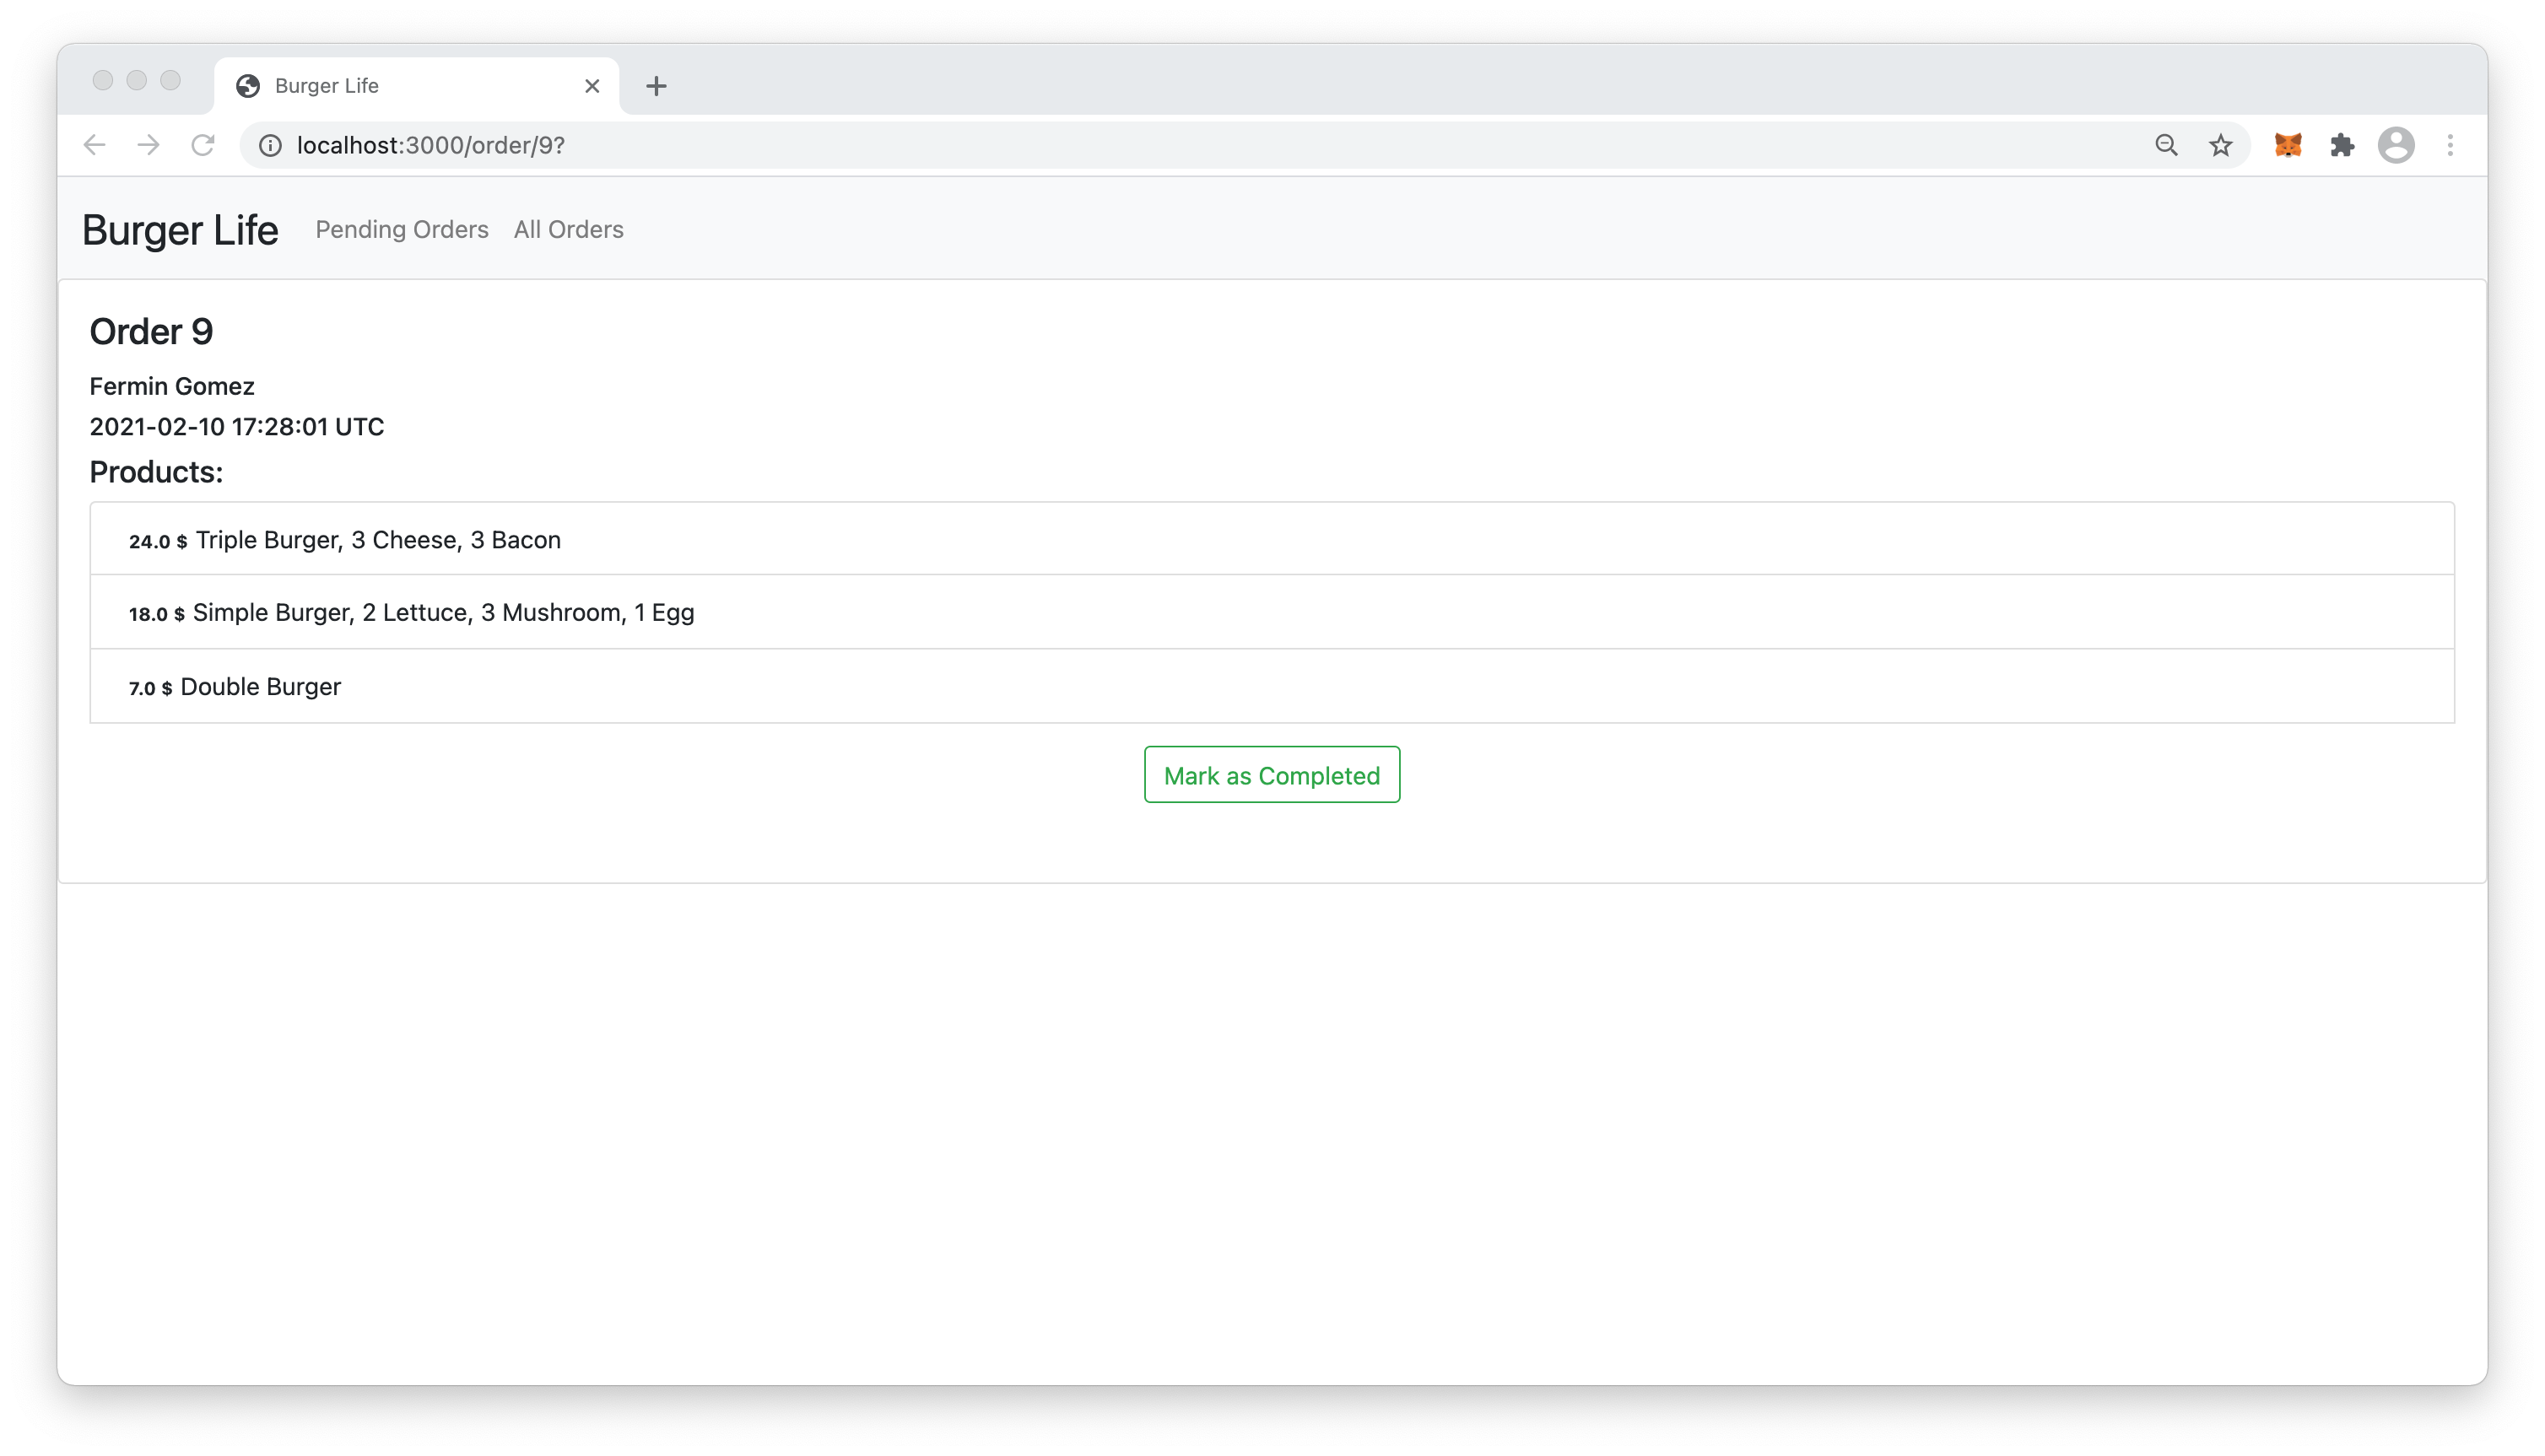
\includegraphics[width=1.0\linewidth]{webapp-order}
\end{figure}

Bajo la sección “All Orders” podremos visualizar el historial completo de pedidos enviados por clientes, como también realizar búsquedas mediante el uso de filtros.

\begin{figure}[H]
	\centering
	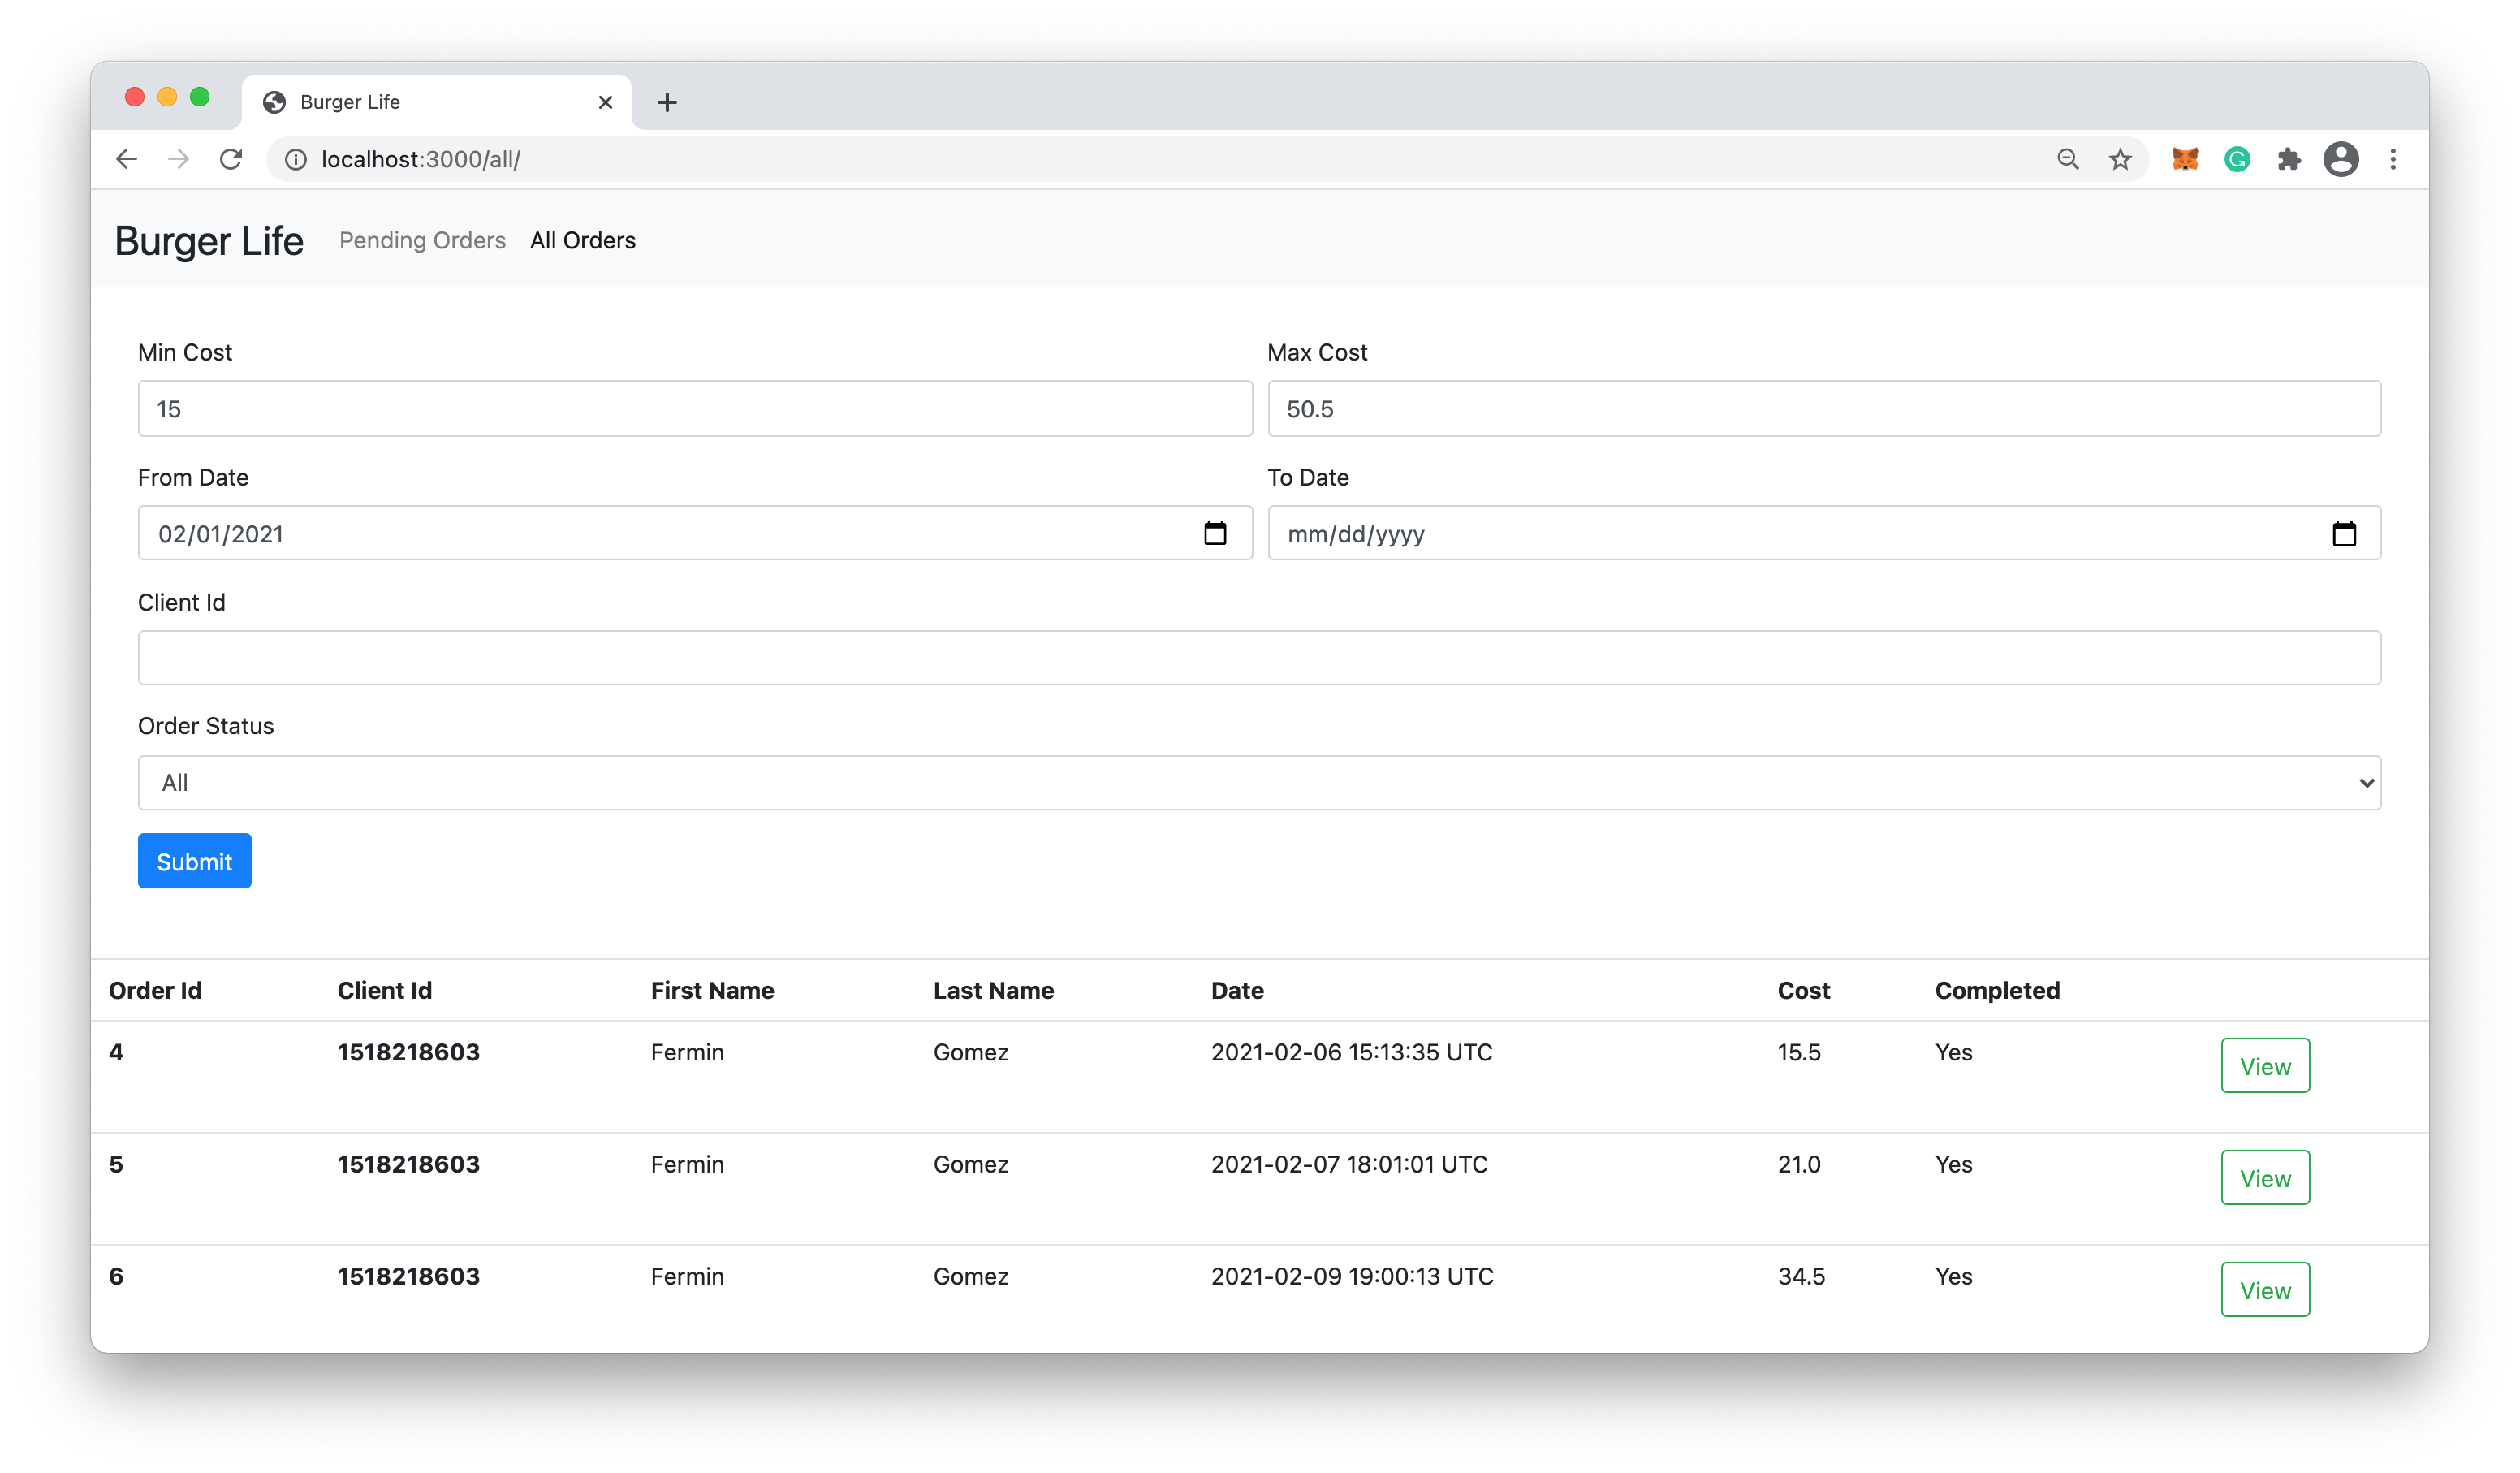
\includegraphics[width=1.0\linewidth]{webapp-search}
\end{figure}

Se podrá filtrar según un rango de fechas, rango de precios, estado de la orden (completada, no completada o ambas) y por último utilizando el identificador del cliente que coincide con el de identificador de telegram.

\pagebreak

\section{Arquitectura}

\subsection{Modelos}

En esta sección no se detallaran todos los modelos utilizados sino que aquellos comunes tanto para el chatbot como para la aplicación web.
\\
Se definió un tipo nuevo \textbf{Burger} que nos permite expresar una hamburguesa y otro tipo \textbf{Topping} para expresar los ingredientes adicionales en Haskell.

\begin{minted}{haskell}
data Burger = Layer Int Topping Burger | Simple | Double | Triple 
	deriving (Show, Eq, Read)
data Topping = Tomato | Cheese | Egg | Onion | Bacon | Lettuce | Pickle |
	Mushroom | Mayo | Ketchup | Mustard  
	deriving (Show, Eq, Read)
\end{minted}

Una hamburguesa puede ser simple, doble o triple. A su vez se le pueden agregar capas con una cantidad específica de ingredientes que la hacen más rica.

\subsection{Chatbot	}

A la hora de implementar el chatbot se tuvo decidir entre las plataformas WhatsApp y Telegram. Por un lado WhatsApp es la aplicación de mensajería más adoptada a nivel global y la que utiliza Arredondo para comunicarse con sus clientes. A diferencia de Telegram no es una aplicación popular, sin embargo telegram-bot-simple \cite{telegram-bot-simple} es una librería escrita en Haskell basada en Telegram Bot API \cite{telegram-bot-api} que nos permite crear bots para Telegram. Por estas razón se optó por desarrollar el chatbot en Telegram.
\\
Telegram-bot-simple requiere de definir dos tipos en Haskell. Uno al cual nombramos \textbf{BotModel} que representa el estado de una conversación del bot. El representa las acciones que ejecuta el bot, a el cual nombramos \textbf{Action}.

\begin{minted}{haskell}
data BotModel = BotModel {
	burgers         :: [Burger],
	currentBurger   :: Maybe Burger,
	prices          :: Prices
} deriving (Show)

data Action = DoNothing | Start  | BurgerMenu | ToppingMenu (Maybe Topping) |
	SauceMenu  | AddBurger Burger | AddTopping Topping Int | Order |
	Confirm (Maybe Client)  | Remove Text  | ShowOrder  | Help  
	deriving (Show, Read)
\end{minted}

A la hora de crear nuestro \textbf{BotApp}, el constructor de la librería requiere de 4 parámetros.

\begin{itemize}
	\item \textbf{botInitialModel}: Estado inicial del bot (\textbf{BotModel}).
	\item \textbf{botAction}: Toma updates de Telegram [link] y los convierte en acciones (\textbf{Action}).
	\item \textbf{botHandler}: Maneja las acciones emitidas (Action), retorna un nuevo estado de conservación del bot (\textbf{BotModel}) y la próxima a acción a realizar.
	\item \textbf{botJobs}: Lista de trabajos a ejecutar según un cronograma. No utilizaremos esta funcionalidad.
\end{itemize}

burgersPrices y toppingPrices son listas de tipo  [(Burger, Double)] y [(Topping, Double)] respectivamente. Almacena los precios correspondientes a cada ingrediente adicional y tamaño de hamburguesa. Estos precios son tomados mediante una consulta a la base de datos. Se decidió tomar estos valores cada vez 

\begin{minted}{haskell}
getBot :: IO (BotApp BotModel Action)
getBot = do
burgersPrices <- selectBurgersPrices
toppingsPrices <- selectToppingsPrices
let bot = BotApp  { botInitialModel = BotModel [] Nothing $ Prices toppingsPrices burgersPrices
	, botAction = flip handleUpdate
	, botHandler = handleAction
	, botJobs = []  }
return bot    
\end{minted}
	
Las acciones del bot pueden ser accionadas mediante comandos enviados como mensaje de texto por el usuario o por una acción de callback llamada al cliquear alguno de los botones disponibles en el inline chat.

\begin{minted}{haskell}
handleUpdate :: BotModel ->  Telegram.Update -> Maybe Action
handleUpdate _model update = (parseUpdate
$  BurgerMenu                    <$    command "menu" 
<|> Start                         <$    command "start" 
<|> ShowOrder                     <$    command "show" 
<|> Remove                        <$>   command "remove"
<|> Confirm (getOrderData update) <$    command "confirm"
<|> callbackQueryDataRead
<|> Help                          <$    (command "help" <|> text)) update
\end{minted}

\pagebreak

A continuación detallaremos sobre el diseño de cada acción.

\begin{itemize}
	\item 
	\textbf{DoNothing}: No altera el estado del bot y no emite ninguna próxima acción a ejecutar
	
	\item
	\textbf{Start}: Accionado con el comando 
	\color{blue}\uline{\textbackslash start}\color{black}
	. No altera el estado del bot, envía como mensaje de texto al usuario un mensaje de bienvenida, su próxima acción es DoNothing.
	
	\item
	\textbf{BurgerMenu}: Accionado con el comando 
	\color{blue}\uline{\textbackslash menu}\color{black}
	. No altera el estado del bot. Comienza el proceso de creación de la hamburguesa enviando al usuario una serie de botones en formato inline chat para seleccionar el tamaño deseado de su hamburguesa. Su próxima acción es DoNothing.
	
	\item
	\textbf{AddBurger  \color{blue}Burger\color{black}}: Accionado como callback al cliquear sobre un botón inline de tamaño de hamburguesa. Almacena la hamburguesa seleccionada en la variable currentBurger de nuestro BotModel y lo retorna como nuevo estado.  Su próxima acción es ToppingMenu.
	
	\item
	\textbf{ToppingMenu \color{blue}(Maybe Topping)\color{black}}: No altera el estado del bot. Envía al usuario una serie de botones en formato inline chat para seleccionar los ingredientes adicionales, cliquear en uno se despliega una nueva serie de botones que permiten elegir la cantidad del mismo. Su próxima acción es DoNothing.
	
	\item
	\textbf{SauceMenu}: No altera el estado del bot. Funciona como una extensión del menú de ingredientes adicionales así evitar el extenso contenido en un mismo lugar. Aquí solo se encuentran las salsas, por lo que envía al usuario una serie de botones en formato inline chat para seleccionar la salsa deseada. Su próxima acción es DoNothing.
	
	\item
	\textbf{AddTopping \color{blue}Topping Int\color{black}}: Accionado como callback una vez seleccionado el ingrediente adicional y su cantidad en el menú de botones inline. Modifica el estado de nuestro BotModel agregando una capa a la hamburguesa almacenada en la variable currentBurger y lo retorna como nuevo estado.  Su próxima acción es ToppingMenu, así el usuario puede seguir agregando más ingredientes a su hamburguesa.
	
	\item
	\textbf{Order}: Accionado como callback una vez que no se desean agregar más ingredientes adicionales a la hamburguesa, es decir ya está creada según las preferencias del usuario y queremos agregarla a nuestro pedido. Almacena la hamburguesa creada en la lista burgers de nuestro BotModel y lo retorna como nuevo estado. Responde con un mensaje de confirmación al usuario y su próxima acción es DoNothing.
	
	\item
	\textbf{Confirm \color{blue}(Maybe Client)\color{black}}: Accionado con el comando 
	\color{blue}\uline{\textbackslash confirm}\color{black}
	. Persiste la orden creada por el usuario. Responde con un mensaje de confirmación al usuario y resetea el estado del bot. Su próxima acción es DoNothing.
	
	\item
	\textbf{Remove \color{blue}Text\color{black}}: Accionado con el comando 
	\color{blue}\uline{\textbackslash remove <id>}\color{black}
	. Altera el modelo la quitando de la lista burgers la hamburguesa indicada por parametro.su próxima acción es ShowOrder. 
	
	\item
	\textbf{ShowOrder}: Accionado con el comando 
	\color{blue}\uline{\textbackslash show}\color{black}
	. No altera el estado del bot, envía como mensaje de texto al usuario todas las hamburguesas de su orden y su precio. Su próxima acción es DoNothing.
	
	\item
	\textbf{Help}: Accionado con el comando 
	\color{blue}\uline{\textbackslash help}\color{black}
	 o al realizar cualquier otra acción que no corresponda a la de un comando. No altera el estado del bot, envía como mensaje de texto al usuario un mensaje de ayuda, su próxima acción es DoNothing. 
	
\end{itemize}

A la hora de diseñar las acciones y su efecto, el tipo BotModel e implementar la función handleAction se tuvo que optar por incluir en BotModel la variable currentBurger. Esta decisión se tomó debido a que telegram-bot-simple permite un máximo de 64 bytes a ser enviados en una acción de callback. Si deseamos enviar el dato currentBurger como parámetro en una acción de callback la cantidad de ingredientes adicionales a agregar sería limitada.

\subsection{Aplicación Web}

Se decidió implementar el mecanismo de seguimiento de los pedidos como una aplicación web ya que de esta forma se necesitan pocos requerimientos por parte del restaurante para comenzar a implementar el sistema. Basta un dispositivo con acceso a internet y un browser para poder utilizarlo, ya sea este una computadora o un celular.
\\
Teniendo en cuenta que no era un requerimiento realizar un sistema muy sofisticado. La arquitectura candidata consiste de una aplicación web estática desarrollada en Haskell utilizando una combinación de Spock junto con blaze-html.
\\
Spock \cite{spock} es un framework de desarrollo web, con la ventaja de ser sencillo y permitiendo un rápido desarrollo.
\\
blaze-html \cite{blaze-html} es una biblioteca para incorporar plantillas HTML en el código Haskell para una eficiencia y capacidad de composición óptimas.
\\
Las rutas disponibles por la aplicación web son:

\begin{itemize}
	\item 
	\color{blue}“/”\color{black}: Muestra la página principal que contiene los pedidos pendientes.
	\item 
	\color{blue}“/search”\color{black}: Muestra el historial de pedidos.
	\item
	\color{blue}“order/<orderId>”\color{black}: Muestra los productos de una orden.
	\item
	\color{blue}“done/<orderId>”\color{black}: Marca como completada una orden y redirecciona a la página principal
\end{itemize}

\subsection{Persistencia}

A la hora de persistir la información se optó por un modelo relacional y postgreSQL como motor de base de datos.

\begin{figure}[H]
	\centering
	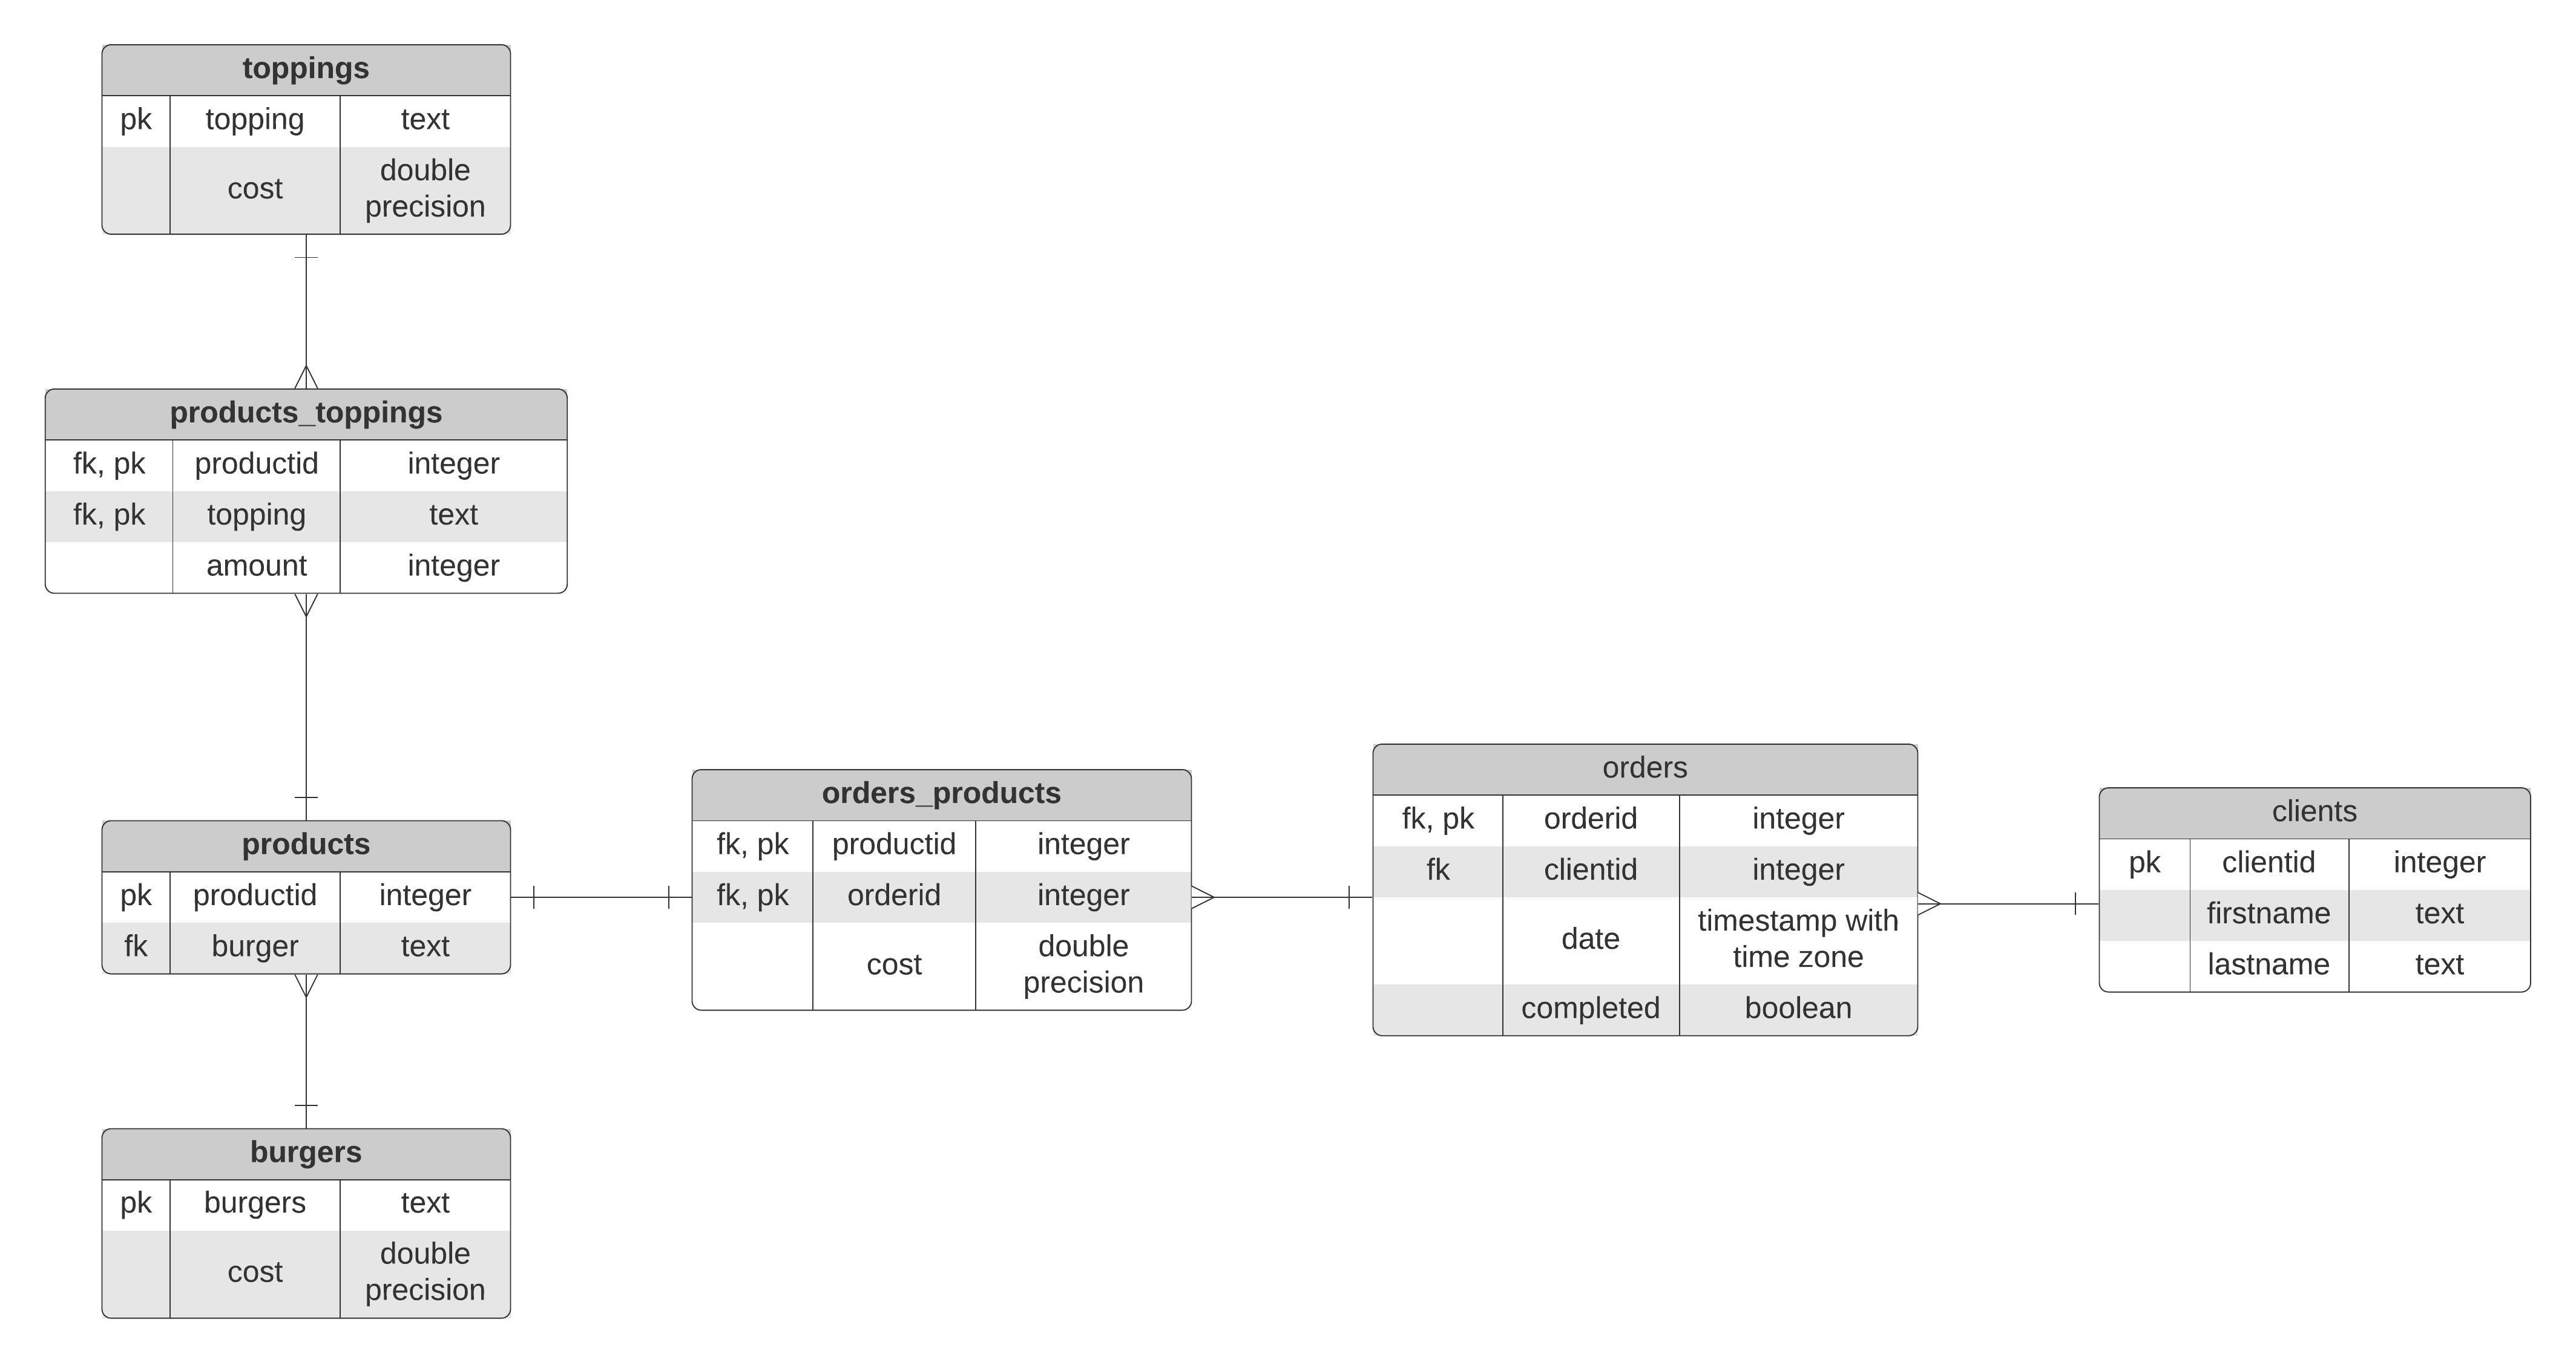
\includegraphics[width=1.0\linewidth]{diagrama-er.jpeg}
\end{figure}

Tanto el chatbot como la aplicación web poseen acceso a la base datos para almacenar datos y realizar las consultas que sean necesarias. 
\\
Las consultas a la base de datos fueron implementadas en Haskell utilizando la librería postgresql-simple \cite{postgresql-simple}.

\pagebreak

\section{Limitaciones y Futuras Extensiones}

\subsection{Chatbot}

Telegram Bot Api permite crear bots que acepten pagos, sin embargo esta funcionalidad aún no fue implementada por la librería telegram-bot-simple. Permitir que Burger bot acepte pagos implicaría poder reducir aún más la circulación y contacto entre personas como también brindar experiencia ágil al comensal.
\\\\
Con el fin de mejorar la experiencia del cliente, el chatbot podría ofrecer mensajes de seguimiento. Como por ejemplo notificarle cuando su pedido comenzó a prepararse en la cocina y cuando está en camino a su mesa.

\subsection{Aplicación Web}

El principal objetivo del proyecto consistió en la realización del chatbot por lo que se buscó que la aplicación web sea sencilla y de rápido desarrollo. Carece de diversas funcionalidades como por ejemplo credenciales de acceso para los empleados del restaurante.

\section{Conclusiones}

\nocite{postgres-simple-tutorial}
\nocite{postgresql-simple-examples}
\nocite{fizruk-telegram-bot-simple}
\nocite{lambda-conf-1}
\nocite{lambda-conf-2}
\nocite{spock-tutorial}
\nocite{blaze-html-tutorial}
\bibliographystyle{plainurl}
\bibliography{References}

\end{document}
